\documentclass{article}
\usepackage[utf8]{inputenc}

\title{Assignment Template}
\author{Brian Kelly}
\date{February 2021}

\usepackage{natbib}
\usepackage{graphicx}
\usepackage{hyperref}

% WHaaaaaaa, is this a comment?!
% Bet you can't do headers and foot... oh my
\usepackage[headsepline=0.005pt:,footsepline=0.005pt:,
plainfootsepline,automark]{scrlayer-scrpage}
\clearpairofpagestyles
\ohead[]{\headmark} \ofoot[\pagemark]{\pagemark}
\ModifyLayer[addvoffset=-.6ex]{scrheadings.foot.above.line}
\ModifyLayer[addvoffset=-.6ex]{plain.scrheadings.foot.above.line}
\setkomafont{pageheadfoot}{\small}

%For graph
\usepackage{tikz}

\begin{document}

\maketitle

\section{Introduction}
This should be a fun intro to using LaTeX.\\
There is a theory which states that if ever anyone discovers exactly what the Universe is for and why it is here, it will instantly disappear and be replaced by something even more bizarre and inexplicable.
There is another theory which states that this has already happened.

Where to find a \href{http://tug.ctan.org/info/latex-refsheet/LaTeX_RefSheet.pdf}{cheatsheet} \leq -Link

\subsection{This is kind of relevant to the intro, but not}
This subsection has to due with the section, but does not have enough content to warrant its own section.\\ What?!?! How did I create a new line

\section{Graph}
Woaow, this is pretty rad\\
\begin{tikzpicture}
  [scale=.8,auto=left,every node/.style={circle,fill=blue!20}]
  \node (n6) at (1,10) {6};
  \node (n4) at (4,8)  {4};
  \node (n5) at (8,9)  {5};
  \node (n1) at (11,8) {1};
  \node (n2) at (9,6)  {2};
  \node (n3) at (5,5)  {3};

  \foreach \from/\to in {n6/n4,n4/n5,n5/n1,n1/n2,n2/n5,n2/n3,n3/n4}
    \draw (\from) -- (\to);

\end{tikzpicture}


\section{Image Time}
Please, enjoy this random stock image:
\begin{figure}[h!]
\centering
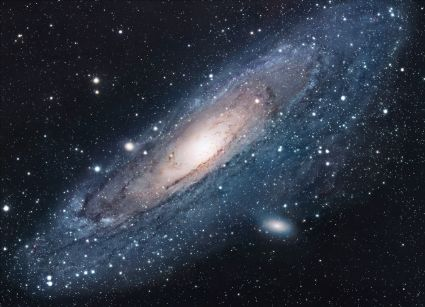
\includegraphics[scale=1.7]{universe}
\caption{The Universe}
\label{fig:universe}
\end{figure}

\section{List Time}
\subsection{Unordered list}
\begin{itemize}
  \item One entry in the list
  \item Another entry in the list
\end{itemize}

\subsection{Ordered List}
\begin{enumerate}
  \item The labels consists of sequential numbers.
  \item The numbers starts at 1 with every call to the enumerate environment.
\end{enumerate}

\section{Nested List}
What?! No! This.... this is too much... A LIST... IN A LIST!
\begin{enumerate}
   \item The labels consists of sequential numbers.
   \begin{itemize}
     \item The individual entries are indicated with a black dot, a so-called bullet.
     \item The text in the entries may be of any length.
   \end{itemize}
   \item The numbers starts at 1 with every call to the enumerate environment.
\end{enumerate}

\section{Pure Madness List}
My mind is blown...
\begin{enumerate}
   \item First level item
   \item First level item
   \begin{enumerate}
     \item Second level item
     \item Second level item
     \begin{enumerate}
       \item Third level item
       \item Third level item
       \begin{enumerate}
         \item Fourth level item
         \item Fourth level item
       \end{enumerate}
     \end{enumerate}
   \end{enumerate}
 \end{enumerate}

\section{Conclusion}
``I always thought something was fundamentally wrong with the universe'' \citep{adams1995hitchhiker}

\bibliographystyle{plain}
\bibliography{references}
\end{document}
